\documentclass[12pt]{article}
\usepackage{verbatim}
\usepackage[dvips]{epsfig}
\usepackage{color}
\usepackage{url}
\usepackage[colorlinks=true]{hyperref}

\begin{document}

\section*{GENESIS: Documentation}

{\bf Related Documentation:}
% start: userdocs-tag-replace-items related-do-nothing
% end: userdocs-tag-replace-items related-do-nothing

\section*{De Schutter: Purkinje Cell Model}

\subsection*{Source}

De Schutter E \& Bower JM (1994) An active membrane model of the cerebellar Purkinje cell I. Simulation of current clamp in slice. {\it Journal of Nerurophysiology}. {\bf 71}: 375--400. \\

\subsection*{Fast and Persistent Sodium Conductances}

\begin{figure}[h]
\centering
   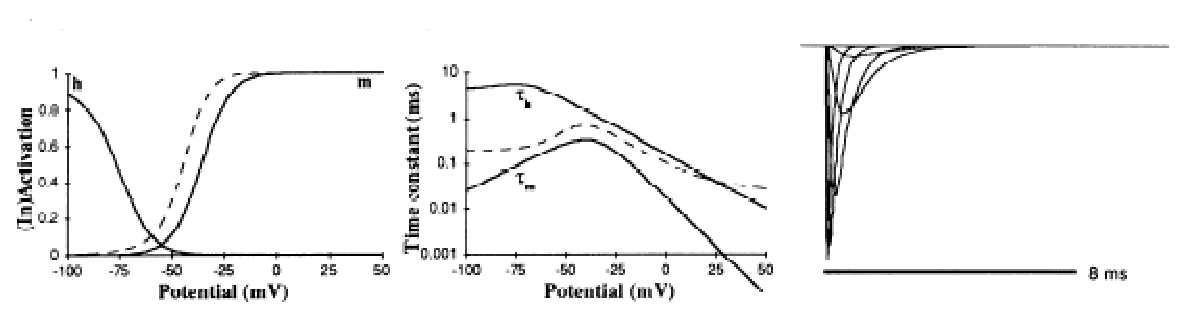
\includegraphics[scale=0.75]{figures/DS1.2A.eps}
   \caption{Activation and inactivation properties of the fast Na$^+$ current (NaF, ---) and persistent Na$^+$ (NaP, - - -, no inactivation) ionic conductances in the model. Seady-state activation and inactivation vs. voltage are plotted at the {\em left}, the time constants of activation ($\tau_m$) and inactivation ($\tau_h$) vs. voltage in the {\em middle} (Note: Semilogarithmic scale), and a simulation of representative voltage-clamp currents at the {\em right}. The voltage-clamp simulation shows the NaF current only. The voltage clamps simulate steps from a holding potential of -110 to -70\,mV up to 0\,mV in 10\,mV increments. The voltage-clamp current amplitude has been scaled arbitrarily because we mainly wanted to demonstrate the current kinetics.}
   \label{fig:DS1.2A}
\end{figure}

\subsection*{Fast Sodium Current}

The fast sodium (NaF) current is responsible for the depolarization phase of the somatic action potential; there are no somatic spikes when this current is blocked by tetrodotoxin (TTX--\,\cite{R:1980ly}). The NaF current is difficult to voltage clamp because of its fast activation kinetics and its large conductance. Until now nobody has attempted a complete voltage-clamp study of this current in Purkinje cells. In modeling papers one can trace an evolution of modifications to the original Hodgkin-Huxley\,\cite{hodgkin52:_quantitative_description} equations\,\cite{W:1991qa, D:1982lh, Wilson:1989ff}. Most of these modifications were, to our knowledge, not based on firm experimental data. We have derived our equations for NaF current from the original Hodgkin-Huxley equations\,\cite{hodgkin52:_quantitative_description}. These were modified to accommodate data about steady-state activation of NaF current obtained from outside-out patch-clamp recordings of cultured Purkinje cells (Fig. 4$B$ in\,\cite{Gahwiler:1989fk}). Another report of whole-cell voltage-clamp recordings from cultured Purkinje cells (Fig. 7$B$ in\,\cite{Hirano:1989uq}) provided a current-voltage (I--V) relation for the peak NaF current with a comparable activation threshold, but corresponding to a somewhat shallower slope of the activation curve. Both reports also contained some data on the time to peak of the NaF current. The modifications based on these two reports resulted in a steeper steady-state activation curve with a higher threshold and slower kinetics (at room temperature) than the original Hodgkin-Huxley equations\,\cite{hodgkin52:_quantitative_description}. Figure 4$B$ in\,\cite{Gahwiler:1989fk} also provided steady-state inactivation data, which resulted in a shallower inactivation curve with slower kinetics.

\subsection*{Persistent Sodium Current}
The persistent sodium (NaP) current is assumed to cause the plateau potentials in the soma described by\,\cite{R:1980ly}. The basis for the equations describing NaP current were single-electrode voltage-clamp recordings of NaP current in guinea pig hippocampal neurons\,\cite{C-R-French:1990uq}. These recordings provided steady-state activation data and we assumed the same number of gates as for the NaF channel\,\cite{hodgkin52:_quantitative_description}. Time constants for activation and deactivation and the threshold of activation for NaP current were obtained from\,\cite{Kay:1990kx}. Note: The NaP current activation follows a slope similar to that of NaF current activation, but with a lower threshold of activation.

\bibliographystyle{plain}
\bibliography{../tex/bib/g3-refs}

\end{document}
